\documentclass[aspectratio=169]{beamer}
\usepackage[utf8]{inputenc}
\usepackage{booktabs}
\usepackage{adjustbox}
\usepackage{amsmath,amssymb,amsthm}
\usepackage{mathtools}
\mathtoolsset{showonlyrefs}

%input{../doc-configuration/math-definitions.tex}
\newcommand{\authorname}{Gonzalo Ortega Carpintero}
\newcommand{\institution}{Universidad Autónoma de Madrid}
\newcommand{\projecttitle}{Convexidad y Desigualdades en Espacios Normados}

\newcommand{\dgmp}{\operatorname{Dgm}_p}
\newcommand{\dgmi}{\operatorname{Dgm}_\infty}
\newcommand{\costp}{\operatorname{cost}_p}
\newcommand{\costi}{\operatorname{cost}_\infty}
\newcommand{\wdp}{\omega_p}
\newcommand{\wdi}{\omega_\infty}
\newcommand{\twdp}{\tilde \omega_p}
\newcommand{\twdi}{\tilde \omega_\infty}
\newcommand{\p}{\mathcal P}
\newcommand{\B}{\mathcal B}
\newcommand{\T}{T_\#}
\newcommand{\N}{\mathbb N}
\newcommand{\Z}{\mathbb Z}
\newcommand{\R}{\mathbb R}
\newcommand{\C}{\mathbb C}
\newcommand{\e}{\varepsilon}
\newcommand{\upr}{\mathbb{R}_<^2}

\newcommand{\barc}{\operatorname{Bar}}
\newcommand{\im}{\operatorname{im}}

\newcommand{\di}{d_{\operatorname{int}}}
\newcommand{\db}{d_{\operatorname{bot}}}
\newcommand{\dhf}{d_{\operatorname{H}}}
\newcommand{\dgh}{d_{\operatorname{GH}}}
\newcommand{\st}{\operatorname{St}}

\newcommand{\cf}{\check{\mathcal{C}}}
\newcommand{\rf}{\mathcal{R}}
\newcommand{\n}{\mathcal{N}}

\usetheme{Madrid}

\definecolor{mycolor}{rgb}{0.5, 0.5, 0.75}
\definecolor{green}{rgb}{0.3, 0.7, 0.3}
\definecolor{grey}{rgb}{0.4, 0.4, 0.4}
\usecolortheme[named=mycolor]{structure}

\useoutertheme{infolines} % Alternatively: miniframes, infolines, split

\setbeamercolor{palette primary}{bg=green,fg=white} % Titulo, derecha
\setbeamercolor{palette secondary}{bg=green,fg=white} % Medio
\setbeamercolor{palette tertiary}{bg=green,fg=white} % Izquierda
\setbeamercolor{structure}{fg=grey} % Fondos y secciones



\title{\projecttitle}
\subtitle{Curso Avanzado de Análisis - \institution}
\author{\authorname}
\date{Martes $27$ de mayo de 2025}

\begin{document}

\frame{\titlepage}

\AtBeginSection[]
{
  \begin{frame}{Contents}
    \tableofcontents[currentsection]
  \end{frame}
}

\section{Espacios convexos}
\subsection{Definiciones}
\begin{frame}
  \frametitle{Espacios convexos}
  \framesubtitle{Definiciones}
  \begin{block}{Definición (Conjunto convexo)}
    Un conjunto $ C \subseteq X $ es {\bf convexo} si para todo par de puntos $ x, y \in C $, $ t \in [0, 1] $, se tiene
    \begin{equation}
      tx + (1-t)y \in C
    \end{equation}
  \end{block}
  \begin{block}{Proposición}
    Sea $ p \colon X \to [0,\infty) $ una función con la propiedad de que para todo $ x \in X $ y para todo $ \lambda \in \R $ se tiene que $ p(\lambda x) = |\lambda| p(x) $. Dicha función satisface la desigualdad triangular si y solo si la bola  $B_p \coloneq \{ x \in X \colon p(x) \leq 1 \} $ es convexa.
  \end{block}
\end{frame}

\begin{frame}
  \begin{block}{Definición (Espacio estrictamente convexo)}
    Un espacio normado $ (X, \| \cdot \|) $ es {\bf estrictamente convexo} si para todo par de puntos $ x $ e $ y $ en la esfera unidad $ S(X) $ tales que el punto medio del segmento que los une esta también en la esfera unidad, i.e. $\| \frac{x+y}{2}\| $, se tiene $ x = y $.
  \end{block}
  \centering
  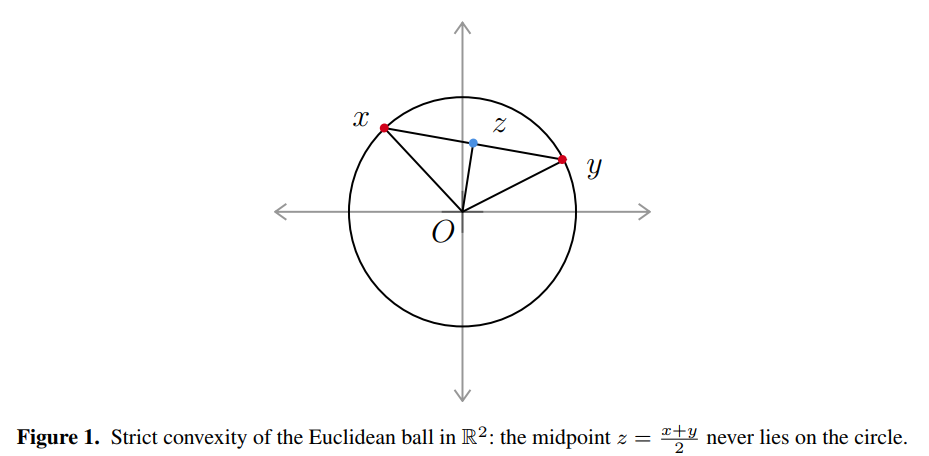
\includegraphics[width=13.5cm]{figures/Screenshot 2025-05-26 201457.png}
\end{frame}

\begin{frame}
  \frametitle{Espacios convexos}
  \framesubtitle{Definiciones}
  \begin{block}{Definición (Espacio uniformemente convexo)}
    Un espacio normado $ (X, \| \cdot \|) $ es {\bf uniformemente convexo} si para todo $ \varepsilon \in (0, 2] $, existe un $ \delta \in (0, 1) $ tal que para todo par $ x, y \in B(X) $ con $ \| x - y \| > \varepsilon $ se tiene $ \| \frac{x+y}{2} \| < \delta $.
  \end{block}
  \centering
  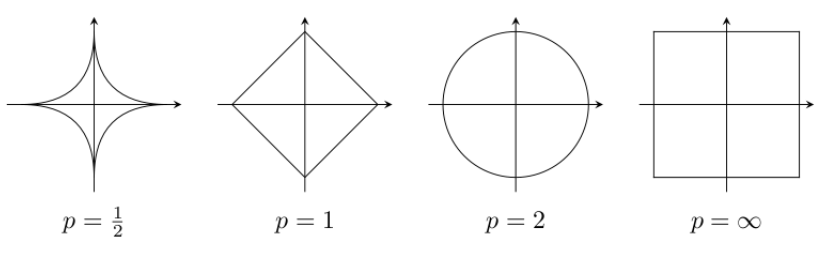
\includegraphics[width=13.5cm]{figures/2.png}
\end{frame}

\begin{frame}
  \frametitle{Espacios convexos}
  \framesubtitle{Motivación}
  \begin{block}{Proposición}
    Para cualquier $\varepsilon \in (0,2]$, existe un $\delta \in (0,1)$ tal que, para todo $x, y \in S(X)$ con $\|x - y\|_2 > \varepsilon$, se tiene que
    \begin{equation}
        \left\| \frac{x + y}{2} \right\|_2 < \delta.
    \end{equation}
  \end{block}
  \begin{block}{Corolario}
    Todo espacio uniformemente convexo es estrictamente convexo.
  \end{block}
\end{frame}

\subsection{Ejemplos}

\begin{frame}
  \begin{block}{Proposición}
    \frametitle{Espacios convexos}
    \framesubtitle{Ejemplos}
    Sea $ (X, \langle \cdot, \cdot \rangle) $ un espacio dotado de un producto escalar con norma $ \|x\| \coloneq \sqrt{\langle x, x \rangle} $. Entonces el espacio $ (X, \|\cdot\|) $ es un espacio uniformemente convexo.
  \end{block}
  La identidad del paralelogramo para normas inducidas por un producto escalar afirma
    \begin{equation}
        \|x + y\|^2 + \|x - y\|^2 = 2(\|x\|^2 + \|y\|^2).
    \end{equation}
\end{frame}

\begin{frame}
  \frametitle{Espacios convexos}
    \framesubtitle{Ejemplos}
    Sea \(x, y \in X\) con \(\|x\| = \|y\| = 1\) y \(x \neq y\). Definimos \(z = \frac{x + y}{2}\).  
    Entonces
    \begin{equation}
    \|z\|^2 = \left\|\frac{x + y}{2}\right\|^2 = \frac{1}{4} \|x + y\|^2.
    \end{equation}
    Aplicando la identidad del paralelogramo tenemos
    \begin{equation}
    \|x + y\|^2 = 2(\|x\|^2 + \|y\|^2) - \|x - y\|^2 = 4 - \|x - y\|^2.
    \end{equation}
    Por lo tanto,
    \begin{equation}
    \|z\|^2 = \frac{1}{4}(4 - \|x - y\|^2) = 1 - \frac{1}{4} \|x - y\|^2.
    \end{equation}
    Como \(x \neq y\), tenemos que \(\|x - y\| > 0\), lo cual implica $ \|z\| < 1 $.
\end{frame}

\begin{frame}
  \frametitle{Convexidad}
  \framesubtitle{Contraejemplos}
  \begin{block}{Observación}
    La convexidad estricta no implica la convexidad uniforme.
  \end{block}
  Consideremos la norma en el espacio de sucesiones convergentes $ \ell^1 $ dada por la suma de las normas $ \ell^1 $ y $ \ell^2 $, es decir, dada una sucesión $ x \in \ell^1 $,
    \begin{equation}
        \| x \| \coloneq \| x \|_{\ell^1} + \| x \|_{\ell^2}.
    \end{equation}
  para todo $ x \neq y \in S(\ell^2) $,
    \begin{equation}
        \|x+y\|_{\ell^2} < \|x\|_{\ell^2} + \|y\|_{\ell^2}.
    \end{equation}
    Por tanto, haciendo también uso de la desigualdad triangular estándar en $ \ell^1 $ tenemos
    \begin{equation}
        \|x+y\| = \|x+y\|_{\ell^1} + \|x+y\|_{\ell^2} < \left( \|x\|_{\ell^1} + \|y\|_{\ell^1} \right) + \left( \|x\|_{\ell^2} + \|y\|_{\ell^2} \right) = \|x\| + \|y\| = 2.
    \end{equation}
    Por tanto, $ \ell_1 $ es estrictamente convexo. 
\end{frame}

\begin{frame}
  Sin embargo, definamos ahora las sucesiones
    \begin{align}
        x_{N, k} &=
        \begin{cases}
            1 & \text{si } k \leq N, \\
            0 & \text{en caso contrario},
        \end{cases}
        &
        y_{N, k} &=
        \begin{cases}
            1 & \text{si } N < k \leq 2N, \\
            0 & \text{en caso contrario}.
        \end{cases}
    \end{align}
    Por un lado tenemos que $ \|x\| = \|y\| = N + \sqrt{N} $ y que $ \|x_N - y_N\| = 2N + \sqrt{2N} $, ya que
    \begin{equation}
        x_{N, k} - y_N =
        \begin{cases}
            1 & \text{si } k \leq N, \\
            -1 & \text{si } N < k \leq 2N, \\
            0 & \text{si } k \geq 2N.
        \end{cases}
    \end{equation}
    Pero tenemos también que
    \begin{equation}
        \left\| \frac{x_N+y_N}{2} \right\| = \frac{2N}{2} + \frac{\sqrt{2N}}{2}.
    \end{equation}
    Dividiendo entre $ N + \sqrt{N} $ podemos hacer $ \left\| \frac{x_N+y_N}{2 (N + \sqrt{N})} \right\| $ tan cercano como queramos a $ 1 $, mientras que siempre tendremos $ \left\| \frac{x_N+y_N}{(N + \sqrt{N})} \right\| \geq \sqrt{2}$. Por tanto, $ (\ell^1, \| \cdot \|) $ no es uniformemente convexo.
\end{frame}

\begin{frame}
  \frametitle{Convexidad}
  \framesubtitle{Contraejemplos: $ L^1 $}
  Consideremos el espacio \(L^1([0,1], \lambda)\) y definamos, para \(n \in \mathbb{N}\):
  \begin{equation}
      f_n = \chi_{[0,1/n]}, \quad g_n = \chi_{[1-1/n,1]}.
  \end{equation}
  Entonces:
  \begin{equation}
      \|f_n\|_1 = \|g_n\|_1 = \frac{1}{n} \to 0.
  \end{equation}
  Definiendo funciones normalizadas,
  \begin{equation}
      \tilde{f}_n = \frac{f_n}{\|f_n\|_1} = n \chi_{[0,1/n]}, \quad \tilde{g}_n = \frac{g_n}{\|g_n\|_1} = n \chi_{[1-1/n,1]}.
  \end{equation}
  Así
  \begin{equation}
      \|\tilde{f}_n\|_1 = \|\tilde{g}_n\|_1 = 1, \quad \|\tilde{f}_n - \tilde{g}_n\|_1 = 2,
  \end{equation}
  pero,
  \begin{equation}
      \left\|\frac{\tilde{f}_n + \tilde{g}_n}{2}\right\|_1 = \frac{1}{2}(\|\tilde{f}_n\|_1 + \|\tilde{g}_n\|_1) = 1.
  \end{equation}
\end{frame}

\begin{frame}
  \frametitle{Convexidad}
  \framesubtitle{Contraejemplos: $ L^\infty $}
  Consideremos el espacio \(L^\infty([0,1], \lambda)\) y definamos:
    \begin{equation}
        f_n = \chi_{[0,1/2]}, \quad g_n = \chi_{[1/2 + 1/n,1]}.
    \end{equation}
    Entonces:
    \begin{equation}
        \|f_n\|_\infty = \|g_n\|_\infty = 1, \quad \|f_n - g_n\|_\infty = 1.
    \end{equation}
    Sin embargo:
    \begin{equation}
        \left\|\frac{f_n + g_n}{2}\right\|_\infty = \frac{1}{2}.
    \end{equation}
  Dado que esta cota no mejora al aumentar \(n\), no es posible encontrar un \(\delta(\epsilon)\) que garantice la disminución necesaria para todo \(\epsilon\). Esto contradice la definición de convexidad uniforme.  
  Por lo tanto, \(L^\infty\) tampoco es uniformemente convexo.  
\end{frame}

\section{Desigualdades}
\subsection{Desigualdades de Clarkson}
\begin{frame}
  \frametitle{Desigualdades}
  \framesubtitle{Clarkson}
  \begin{block}{Teorema}
    Para $ 2 \leq p < \infty $, dadas $ f, g \in L^p $, se verifica la desigualdad
    \begin{equation} \label{eq:clarkson-1}
        \left\| f+g \right\|_p^p + \left\| f-g \right\|_p^p \leq 2^{p-1} \left( \left\|f\right\|_p^p + \left\|g\right\|_p^p \right).
    \end{equation}
  \end{block}
  \begin{block}{Teorema}
    Sea $ 1 < p \leq 2 $, y sea $ q = \frac{p}{p-1}$. Para $ f, g \in L^p $ se tiene
    \begin{equation} \label{eq:clarkson-2}
        \left\| f + g \right\|_p^q + \left\| f - g \right\|_p^q \leq 2 \left(\|f \|_p^p + \|g\|_p^p \right)^{\frac{q}{p}}.
    \end{equation}
  \end{block}
\end{frame}

\begin{frame}
  \frametitle{Desigualdades}
  \framesubtitle{Convexidad uniforme en $L^p$}
  Sean $ f, g \in L^p $ con $ \|f\| = \|g\| = 1 $. Para $ p \geq 2 $, haciendo uso de \eqref{eq:clarkson-1} tenemos
    \begin{equation}
        \| f + g \|_p^p + \| f - g \|_p^p \leq 2^{p-1}(1 + 1) = 2^p.
    \end{equation}
    Ahora, si se tiene $\|f-g\| > \varepsilon \in (0, 2] $, dividiendo entre $ 2^p $ a ambos lados y despejando adecuadamente se sigue
    \begin{equation}
        \left\| \frac{f + g}{2} \right\|_p \leq \left( 1 - \left\| \frac{f - g}{2} \right\|_p^p\right)^{\frac{1}{p}} \leq \left( 1 - \left( \frac{\varepsilon}{2} \right)^p\right)^{\frac{1}{p}} \eqcolon \delta,
    \end{equation}
    donde $ \delta \in (0, 1) $ y se verifica la convexidad uniforme para $ p \geq 2 $. 
\end{frame}

\begin{frame}
  \frametitle{Desigualdades}
  \framesubtitle{Convexidad uniforme en $L^p$}
  Para $ 1 < p \leq 2 $ usamos la desigualdad \eqref{eq:clarkson-2} para obtener
    \begin{equation}
        \left\| f + g \right\|_p^q + \left\| f - g \right\|_p^q \leq 2 \left(\|f \|_p^p + \|g\|_p^p \right)^{\frac{q}{p}}.
    \end{equation}
    Análogamente al procedimiento anterior, ahora con $ \delta \coloneq  \left( 1 - \left( \frac{\varepsilon}{2} \right)^q\right)^{\frac{1}{q}} $ vemos que se verifica la convexidad uniforme también para $ 1 < p \leq 2 $.
\end{frame}

\subsection{Desigualdades de Hanner}

\begin{frame}
  \frametitle{Desigualdades}
  \framesubtitle{Hanner}
  \begin{block}{Teorema}
    Sean $ f $ y $ g $ dos funciones en $L^p$. Para $ p \geq 2 $, se verifica
    \begin{equation} \label{eq:hanner}
        \left\| f+g \right\|_p^p + \left\| f-g \right\|_p^p \leq \left( \|f \|_p + \|g\|_p \right)^p + \left| \|f \|_p - \|g\|_p \right|^p.
    \end{equation}
    Para $ 1 < p \leq 2 $, la desigualdad se invierte.
  \end{block}
\end{frame}

\subsection{Una comparación}

\begin{frame}
  \frametitle{Desigualdades}
  \framesubtitle{Una comparación}
  Dadas $f, g \in L^p $, tomamos las funciones constantes $ f' = \|f \|_p $ y $ g' = \|g\|_p $ donde, naturalmente, $ f', g' \in L^p $ y
  \begin{align}
      \left( \|f \|_p + \|g\|_p \right)^p = \left( f' + g' \right)^p = \left\| f'+g' \right\|_p^p, \\
      \left| \|f \|_p - \|g\|_p \right|^p = \left| f' - g' \right|^p = \left\| f'-g' \right\|_p^p.
  \end{align}
  Así pues, utilizando tanto Clarkson como Hanner, obtenemos la siguiente cadena de desigualdades, probando la mejor cota dada por Hanner:
  \begin{align}
      \left\| f+g \right\|_p^p + \left\| f-g \right\|_p^p &\leq  \left( \|f \|_p + \|g\|_p \right)^p + \left| \|f \|_p - \|g\|_p \right|^p = \left\| f'+g' \right\|_p^p + \left\| f'-g' \right\|_p^p \\
      &\leq 2^{p-1} \left( \|f'\|_p^p + \|g'\|_p^p \right) = 2^{p-1} \left( \|f\|_p^p + \|g\|_p^p \right).
  \end{align}
\end{frame}


\end{document}
